\documentclass{article}

\usepackage{tikz}
\usepackage[inner=0.5cm,outer=0.5cm]{geometry}

\begin{document}
\subsection*{12 faces, wild colouring}
 \bigskip

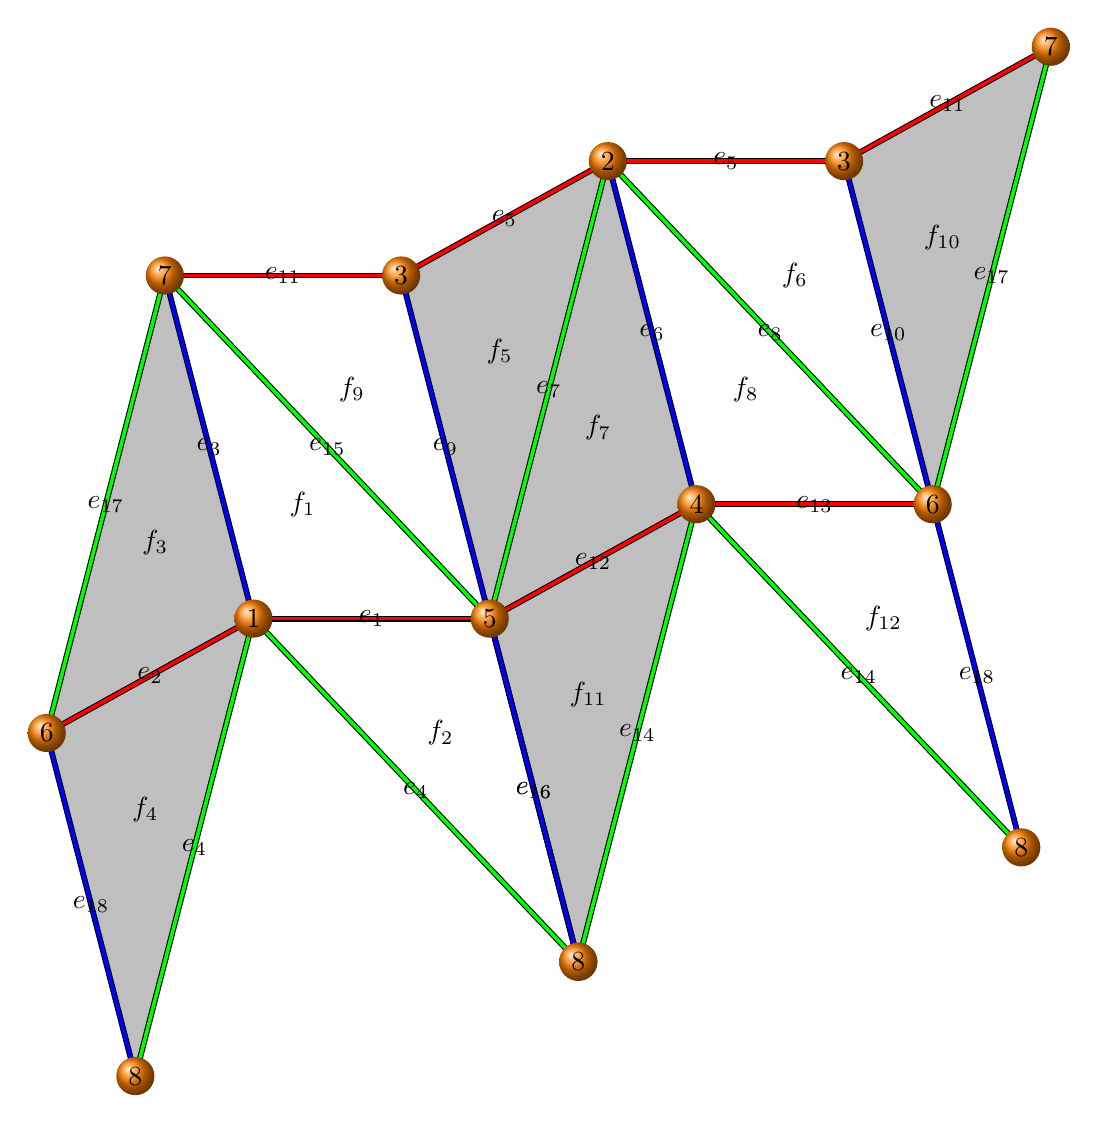
\begin{tikzpicture}[scale=3/2]
\coordinate (V1_1) at (0, 0);
\coordinate (V2_1) at (3, 3.872983346207417);
\coordinate (V3_1) at (1.25, 2.904737509655563);
\coordinate (V3_2) at (5, 3.872983346207417);
\coordinate (V4_1) at (3.75, 0.968245836551854);
\coordinate (V5_1) at (2, 0);
\coordinate (V6_1) at (-1.75, -0.9682458365518543);
\coordinate (V6_2) at (5.75, 0.9682458365518536);
\coordinate (V7_1) at (-0.75, 2.904737509655563);
\coordinate (V7_2) at (6.75, 4.841229182759271);
\coordinate (V8_1) at (2.75, -2.904737509655563);
\coordinate (V8_2) at (-1, -3.872983346207417);
\coordinate (V8_3) at (2.75, -2.904737509655563);
\coordinate (V8_4) at (6.499999999999999, -1.936491673103709);


\fill[white] (V1_1) -- (V5_1) -- (V7_1) -- cycle;
\node (F1) at (0.4166666666666666, 0.9682458365518543) {$f_{1}$};
\fill[white] (V1_1) -- (V5_1) -- (V8_1) -- cycle;
\node (F2) at (1.583333333333333, -0.9682458365518543) {$f_{2}$};
\fill[lightgray] (V1_1) -- (V6_1) -- (V7_1) -- cycle;
\node (F3) at (-0.8333333333333333, 0.6454972243679029) {$f_{3}$};
\fill[lightgray] (V1_1) -- (V6_1) -- (V8_2) -- cycle;
\node (F4) at (-0.916666666666667, -1.613743060919757) {$f_{4}$};
\fill[lightgray] (V2_1) -- (V3_1) -- (V5_1) -- cycle;
\node (F5) at (2.083333333333333, 2.25924028528766) {$f_{5}$};
\fill[white] (V2_1) -- (V3_2) -- (V6_2) -- cycle;
\node (F6) at (4.583333333333333, 2.904737509655562) {$f_{6}$};
\fill[lightgray] (V2_1) -- (V4_1) -- (V5_1) -- cycle;
\node (F7) at (2.916666666666667, 1.613743060919757) {$f_{7}$};
\fill[white] (V2_1) -- (V4_1) -- (V6_2) -- cycle;
\node (F8) at (4.166666666666666, 1.936491673103708) {$f_{8}$};
\fill[white] (V3_1) -- (V5_1) -- (V7_1) -- cycle;
\node (F9) at (0.8333333333333333, 1.936491673103709) {$f_{9}$};
\fill[lightgray] (V3_2) -- (V6_2) -- (V7_2) -- cycle;
\node (F10) at (5.833333333333333, 3.227486121839514) {$f_{10}$};
\fill[lightgray] (V4_1) -- (V5_1) -- (V8_3) -- cycle;
\node (F11) at (2.833333333333333, -0.6454972243679028) {$f_{11}$};
\fill[white] (V4_1) -- (V6_2) -- (V8_4) -- cycle;
\node (F12) at (5.333333333333333, -5.921189464667501e-16) {$f_{12}$};


\tikzset{EdgeStyle/.style = {thin, double distance=1.3pt} }

\draw[ EdgeStyle, double=red] (V5_1) -- node { $e_{1}$ } (V1_1);
\draw[ EdgeStyle, double=red] (V1_1) -- node { $e_{2}$ } (V6_1);
\draw[ EdgeStyle, double=blue] (V1_1) -- node { $e_{3}$ } (V7_1);
\draw[ EdgeStyle, double=green] (V8_1) -- node { $e_{4}$ } (V1_1);
\draw[ EdgeStyle, double=green] (V1_1) -- node { $e_{4}$ } (V8_2);
\draw[ EdgeStyle, double=red] (V3_1) -- node { $e_{5}$ } (V2_1);
\draw[ EdgeStyle, double=red] (V2_1) -- node { $e_{5}$ } (V3_2);
\draw[ EdgeStyle, double=blue] (V2_1) -- node { $e_{6}$ } (V4_1);
\draw[ EdgeStyle, double=green] (V2_1) -- node { $e_{7}$ } (V5_1);
\draw[ EdgeStyle, double=green] (V2_1) -- node { $e_{8}$ } (V6_2);
\draw[ EdgeStyle, double=blue] (V3_1) -- node { $e_{9}$ } (V5_1);
\draw[ EdgeStyle, double=blue] (V3_2) -- node { $e_{10}$ } (V6_2);
\draw[ EdgeStyle, double=red] (V7_1) -- node { $e_{11}$ } (V3_1);
\draw[ EdgeStyle, double=red] (V3_2) -- node { $e_{11}$ } (V7_2);
\draw[ EdgeStyle, double=red] (V4_1) -- node { $e_{12}$ } (V5_1);
\draw[ EdgeStyle, double=red] (V6_2) -- node { $e_{13}$ } (V4_1);
\draw[ EdgeStyle, double=green] (V4_1) -- node { $e_{14}$ } (V8_3);
\draw[ EdgeStyle, double=green] (V8_4) -- node { $e_{14}$ } (V4_1);
\draw[ EdgeStyle, double=green] (V7_1) -- node { $e_{15}$ } (V5_1);
\draw[ EdgeStyle, double=blue] (V5_1) -- node { $e_{16}$ } (V8_1);
\draw[ EdgeStyle, double=blue] (V8_3) -- node { $e_{16}$ } (V5_1);
\draw[ EdgeStyle, double=green] (V6_1) -- node { $e_{17}$ } (V7_1);
\draw[ EdgeStyle, double=green] (V7_2) -- node { $e_{17}$ } (V6_2);
\draw[ EdgeStyle, double=blue] (V8_2) -- node { $e_{18}$ } (V6_1);
\draw[ EdgeStyle, double=blue] (V6_2) -- node { $e_{18}$ } (V8_4);



\tikzset{VertexStyle/.style = {
 shape = circle,
 ball color = orange,
 text = black,
 inner sep = 2pt,
 outer sep = 0pt,
 minimum size = 10pt} }

\node[VertexStyle] at (V1_1) {1};
\node[VertexStyle] at (V2_1) {2};
\node[VertexStyle] at (V3_1) {3};
\node[VertexStyle] at (V3_2) {3};
\node[VertexStyle] at (V4_1) {4};
\node[VertexStyle] at (V5_1) {5};
\node[VertexStyle] at (V6_1) {6};
\node[VertexStyle] at (V6_2) {6};
\node[VertexStyle] at (V7_1) {7};
\node[VertexStyle] at (V7_2) {7};
\node[VertexStyle] at (V8_1) {8};
\node[VertexStyle] at (V8_2) {8};
\node[VertexStyle] at (V8_3) {8};
\node[VertexStyle] at (V8_4) {8};

\end{tikzpicture}

\end{document} 
